\title{Informe de Estadística en Física Experimental: Ejercicio 6 y 7 Guía 5}
\author{Andr\'es Babino}

\begin{document}
\maketitle
\section{Introducción}
El lenguaje utilizado para programar todas los ítems fue Python.
El código utilizado para generar los datos, gráficos y este mismo informe fue controlado con git, tiene licencia MIT y está almacenado en \url{https://github.com/ababino/efe}.

\section*{Ejercicio 6, ítem d}
Si $y_a=a_1 + a_2 x_a$ entonces el valor esperado de $y_a$ será $E(y_a)=\hat x_1 + \hat x_2 x_a$.
Para calcular su varianza uso la fórmula de propagación de errores:
\begin{equation}
Var(y_a) = \left. \frac{\partial y_a}{\partial a_1}\right|_{\hat a_1, \hat a_2}^2 Var(a_1) + \left. \frac{\partial y_a}{\partial a_2}\right|_{\hat a_1, \hat a_2}^2 Var(a_2) + 2 \left. \frac{\partial y_a}{\partial a_1}\right|_{\hat a_1, \hat a_2} \left. \frac{\partial y_a}{\partial a_2}\right|_{\hat a_1, \hat a_2} Cov(a_1, a_2)
\label{eq:prop}
\end{equation}

usando las definiciones del enunciado:

\begin{equation}
\sigma_a = \sqrt{\frac{\sigma^2}{\Delta} \left(N x_a^2 -2 \sum_{i=1}^N x_i x_a +\sum_{i=1}^N x_i^2\right)}
\label{eq:error}
\end{equation}

En el gráfico de la figura \ref{fig:e6d} se muestran los datos del enunciado, el ajuste lineal y, en linea punteada, el error de ajuste usando la fórmula \ref{eq:error}.

\begin{figure}
\centering
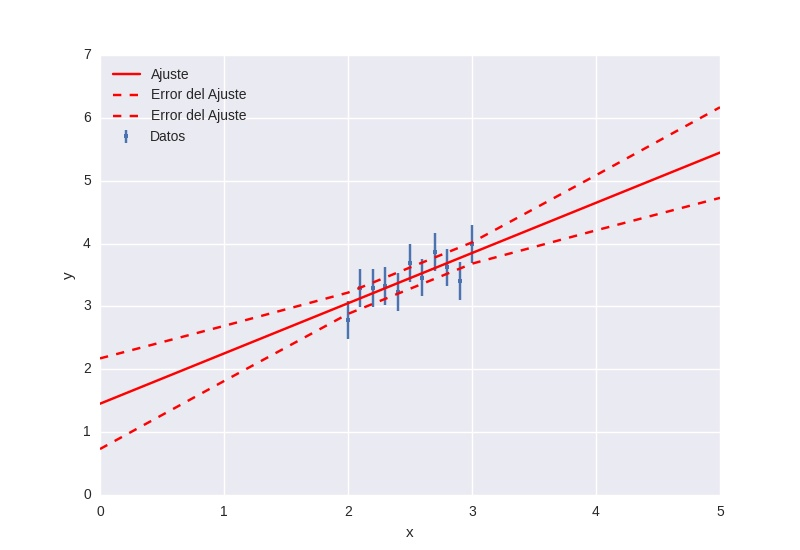
\includegraphics[width=0.75\textwidth]{ej6d.jpg}
\caption[]{}
\label{fig:e6d}
\end{figure}

Cómo $\sigma_a$ es una función cuadrática de $x_a$, para hallar el valor de $x_a$ que minimiza $\sigma_a$ podemos usar la famosa fórmula del vértice de una parábola $\frac{-b}{2a}$:
$$
x_a^{min} = -\frac{\sum_{i=1}^N x_i}{N}
$$

que es justamente el valor medio de las $x$. 
Esto es razonable porque a medida que nos alejamos del centro de los datos tenemos menos información y por lo tanto el error aumenta. 
El mínimo valor de $\sigma_a$ es:

$$
\sigma_a(x_a^{min}) = \frac{\sigma}{\sqrt{N}}
$$

que es exactamente la varianza del promedio.

\section*{Ejercicio 6, ítem e}
Si ignoramos el término de covarianza en la fórmula de propagación de errores (ecuación \ref{eq:prop}) obtenemos la siguiente expresión para $\sigma_a$ 

$$
\sigma_a = \sqrt{\frac{\sigma}{\Delta}(N x_a^2 + \sum_{i=1}^N x_i^2)}
$$

En la figura \ref{fig:e6e} se muestran los datos del enunciado con su ajuste y el error que se obtiene si ignoramos el término de covarianza. 
el resultado es claramente erróneo pues no es posible que, independientemente de los datos el $x$ de mínimo error sea siempre $0$.

\begin{figure}
\centering
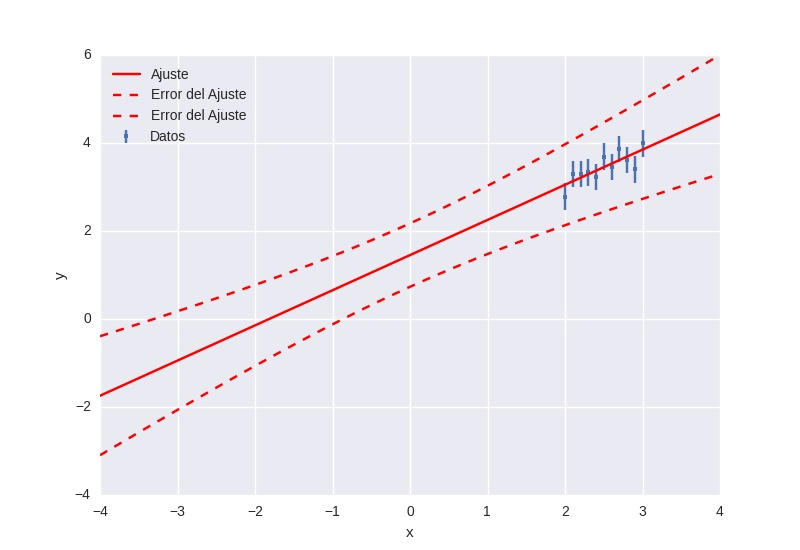
\includegraphics[width=0.75\textwidth]{ej6e.jpg}
\caption[]{}
\label{fig:e6e}
\end{figure}

\section*{Ejercicio 7}
Para verificar los resultados analíticos hallados hasta ahora escribimos un programa que genere 1000 conjunto de datos que provengan de la misma ley lineal.
Con esos mil conjuntos obtenemos 1000 ajustes y con ellos 1000 predicciones $y_a$ par aun dado $x_a=0.5$.
Los resultados de esta simulación se muestran el el gráfico que la figura \ref{fig:e7}.
Las barras azules muestran un histograma (normalizado) de los $y_a$ generados y la linea roja muestra una distribución gaussiana con el valor medio y la varianza teóricas calculadas en el ítem 6d. 

\begin{figure}
\centering
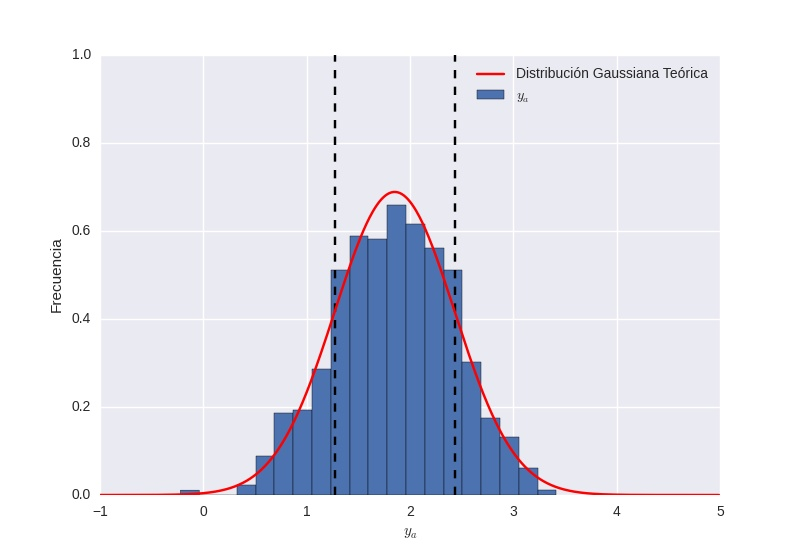
\includegraphics[width=0.75\textwidth]{ej7.jpg}
\caption[]{}
\label{fig:e7}
\end{figure}